%#! lualatex
\documentclass{bxjsarticle}

\usepackage{datetime}
\usepackage{boites}
\usepackage{url}
\usepackage[unicode,hypertexnames=false,bookmarks=false,colorlinks,citecolor=blue,linkcolor=blue,urlcolor=blue]{hyperref}
\usepackage{pdffill}
\usepackage{luajalayout}

\defaultfontfeatures{Ligatures=TeX}

\setrftovf[scale=.95]{IPAexMincho:+jp90}{rmfamily}
\setrftovf[overwrite,exclude=\jarange]{TeX Gyre Termes}{rmfamily}
\setrftovf[scale=.95]{M+ 1c-medium}{rmfamily-B}
\setrftovf[overwrite,exclude=\jarange]{TeX Gyre Termes/B}{rmfamily-B}
\setmainfont[BoldFont=vf:rmfamily-B]{vf:rmfamily}
\setmonofont{m+ 1mn-regular}

\makeatletter
\renewcommand{\section}{\@startsection{section}{1}{\z@}%
   {1.5\Cvs \@plus.5\Cdp \@minus.2\Cdp}%
   {.5\Cvs \@plus.3\Cdp}%
   {\bfseries}}
\makeatother

\begin{document}

\noindent{\large\bfseries pdffill パッケージの説明書} (Last modified: \usdate\today)

\section{概要}

申請書や報告書といった事務書類を作成するとき,慣れない Word や Excel の様式を送ら
れて編集する必要に迫られることが多いです.特にある程度の長さの文章を記述する欄があ
る場合,Word や Excel では無様な仕上がりになってしまったり,枠が崩れてしまったり,
ページ数が不意に増えたりしてイライラします(使い方が下手なせいかもしれないが).
あげくの果てに記入して保存したファイルを修正のためにもう一度開こうとしたらクラッシュ
した日には……(←実体験).

pdffill は使い慣れた \LaTeX で美しく事務書類を作成するためのパッケージです.目標は
科研費 \LaTeX\footnote{\url{http://osksn2.hep.sci.osaka-u.ac.jp/~taku/kakenhiLaTeX/}}の方法を一般化することです.

\section{とりあえず使ってみよう}

細かいことを書く前にまずは使い方を見てみましょう.
例として,次ページにあるような申請書に記入することを考えます.

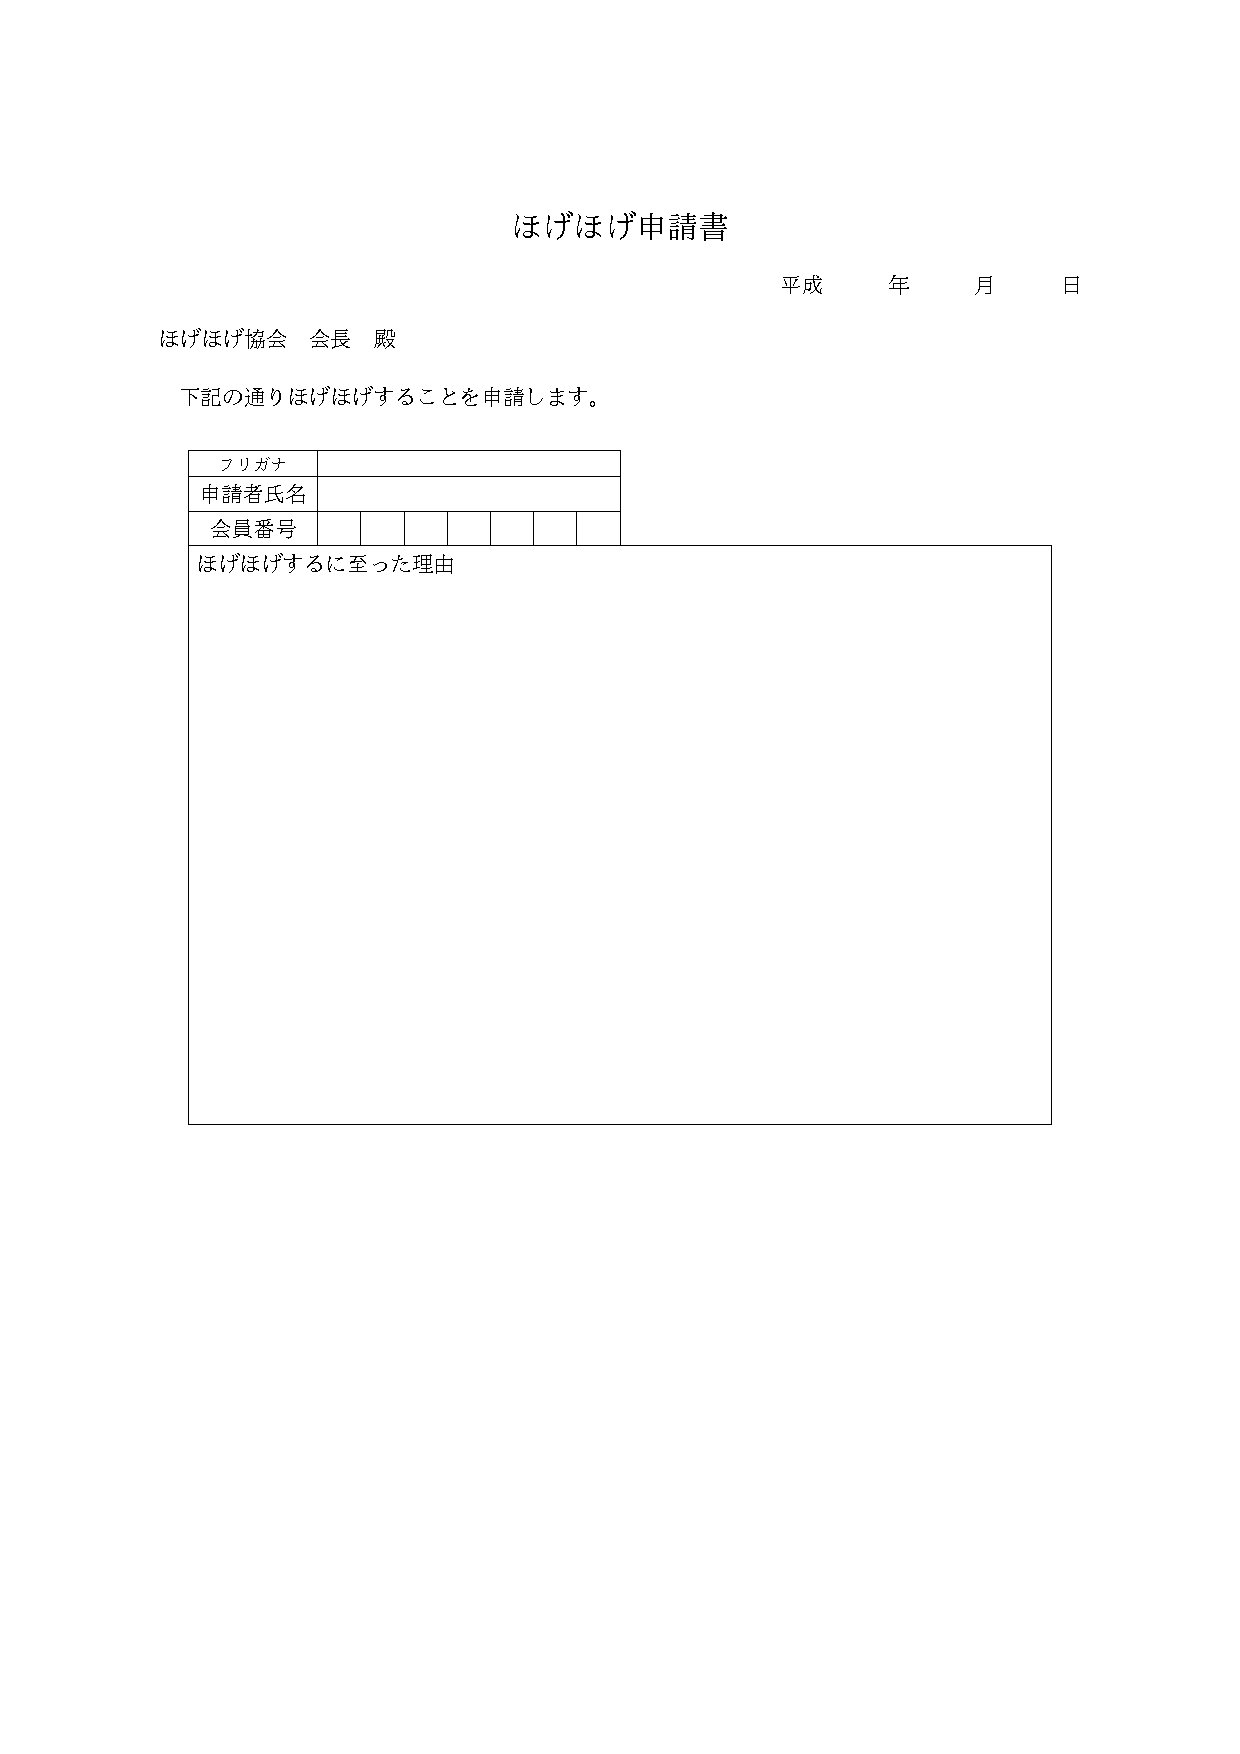
\includepdf{sampleform}

この申請書のファイル名を {\ttfamily sampleform.pdf} とします.
とりあえず,次のように書いたファイルを同じディレクトリに用意しましょう.

\vspace{1em}
\begin{breakbox}
\begin{verbatim}
\documentclass{article}
\usepackage{pdffill}
%% ここに日本語関連のパッケージの読み込み・設定を書く
\begin{document}
\pfdefaultoption{grid,draft}
\pdffill{sampleform}{}
\end{document}
\end{verbatim}
\end{breakbox}
\vspace{1em}

これを {\ttfamily xelatex},もしくは {\ttfamily lualatex} コマンドでコンパイル
すると次ページのような出力が得られます.
出力を見ながら \verb|\pdffill{sampleform}{}| の部分を次のように変えてみましょう.

\long\def\picturecommand{
  % 日付
  \pfnode[right] (13.75, 24.85) {\splitboxes{14.5mm}{{23}{5}{9}}}
  % 名前のフリガナ
  \pfnode[right] (5.6, 21.85) {\footnotesize ホゲ タロウ} 
  % 名前
  \pfnode[right] (5.6, 21.3) {保毛 太郎}                         
  % 会員番号 
  \pfnode[right] (5.38, 20.7) {\splitboxes{7.3mm}{1234567}}        
  % 申請理由
  \pfnode[below right,text width=43em] (3.3, 20) {\parindent=1em\par
    これまでに多くの場でほげほげの経験を積み,その結果あらゆる場面でほげほげする能力を
    身に付けることができました.
    この能力をより広く社会で生かしていくためには,貴協会でほげほげすることが
    何よりも効果的であると判断しました.
    申請が認められた後には,全世界でほげほげするほげほげツアーを実施し,
    さらにほげほげをほげほげしていく所存でほげほげ.

    ほげほげほげほげほげほげほげほげほげほげほげほげほげほげほげほげほげほげほげほげ
    ほげほげほげほげほげほげほげほげほげほげほげほげほげほげほげほげほげほげほげほげ
    ほげほげほげほげほげほげほげほげほげほげほげほげほげほげほげほげほげほげほげほげ
    ほげほげほげほげほげほげほげほげほげほげほげほげほげほげほげほげほげほげほげほげ
    ほげほげほげほげほげほげほげほげほげほげほげほげほげほげほげほげほげほげほげほげ
    ほげほげほげほげほげほげほげほげほげほげほげほげほげほげほげほげほげほげほげほげ
    ほげほげほげほげほげほげほげほげほげほげほげほげほげほげほげほげほげほげほげほげ
    ほげほげほげほげほげほげほげほげほげほげほげほげほげほげほげほげほげほげほげほげ
    ほげほげほげほげほげほげほげほげほげほげほげ?

    ほげほげほげほげほげほげほげほげほげほげほげほげほげほげほげほげほげほげほげほげ
    ほげほげほげほげほげほげほげほげほげほげほげほげほげほげほげほげほげほげほげほげ
    ほげほげほげほげほげほげほげほげほげほげほげほげほげほげほげほげほげほげほげほげ
    ほげほげほげほげほげほげほげほげほげほげほげほげほげほげほげほげほげほげほげほげ
    ほげほげほげほげほげ!
  }  
}

\vspace{1em}
\begin{breakbox}
\begin{verbatim}
\pdffill{sampleform}{
  % 日付
  \pfnode[right] (13.75, 24.85) {\splitboxes{14.5mm}{{23}{5}{9}}}
  % 名前のフリガナ
  \pfnode[right] (5.6, 21.85) {\footnotesize ホゲ タロウ} 
  % 名前
  \pfnode[right] (5.6, 21.3) {保毛 太郎}                         
  % 会員番号 
  \pfnode[right] (5.38, 20.7) {\splitboxes{7.3mm}{1234567}}        
  % 申請理由
  \pfnode[below right,text width=43em] (3.3, 20) {\parindent=1em\par
    これまでに多くの場でほげほげの経験を積み,その結果あらゆる場面でほげほげする能力を
    身に付けることができました.
    この能力をより広く社会で生かしていくためには,貴協会でほげほげすることが
    何よりも効果的であると判断しました.
    申請が認められた後には,全世界でほげほげするほげほげツアーを実施し,
    さらにほげほげをほげほげしていく所存でほげほげ.

    ほげほげほげほげほげほげほげほげほげほげほげほげほげほげほげほげほげほげほげほげ
    (以下略)
  }  
}
\end{verbatim}
\end{breakbox}
\vspace{1em}

これで次々ページの出力が得られます.さらに \verb|\pfdefaultoption{grid,draft}| を
コメントアウトすれば完成です.

\pdffill[grid,draft]{sampleform}{}

\pdffill[grid,draft]{sampleform}{\picturecommand}

\pdffill{sampleform}{\picturecommand}

\section{詳しい使い方}
未完.

\end{document}
